\documentclass[9pt,conference]{IEEEtran}
\usepackage[utf8]{inputenc}
\usepackage[brazil]{babel}

% Diversos
\usepackage{csquotes}
\usepackage{graphicx}
\usepackage{verbatim}
\usepackage{hyperref}
\usepackage{smartdiagram}

% Título
\title{Utilizando Redes Convolucionais de Grafos Espaço-Temporais para o Reconhecimento da Línguas de Sinais}
%\author{Cleison Correia de Amorim}
\date{Outubro 2018}

\author{
    \IEEEauthorblockN{Cleison Correia de Amorim}
    \IEEEauthorblockA{Centro de Informática\\
    Universidade Federal de Pernambuco\\
    Email: cca5@cin.ufpe.br}
}

% Comandos
% 'image': definição de imagem
\newcommand{\image}[4][\linewidth] {
    \begin{figure}[ht]
    \centering
    \includegraphics[width=#1]{#3}
    \caption{#4}
    \label{#2}
    \end{figure}
}

% 'refimage': referências de imagens
\newcommand{\refimage}[1] {figura \ref{#1}}

% 'refsection': referências de seções
\newcommand{\refsect}[1] {seção "\nameref{#1}"}


\begin{document}
\maketitle
\begin{abstract}
The recognition of sign language is a field of research with several challenges, but it has an important role to facilitate the communication of the Deaf and to remove the barriers in this communication to society. This paper presents the application of a deep learning algorithm known as Spatial Temporal Graph Convolutional Network to promote the recognition of this language. This is a new approach centered on human skeletal movement that uses graphs to capture its dynamics in two dimensions, spatial and temporal, and that is able to consider complex aspects of the context of signs. Additionally, this paper presents the creation of a dataset of human skeletons for sign language that is based on ASLLVD, and which, in addition to being used in this study, is publicly available to contribute to future related studies.

%O reconhecimento de sinais é uma área de pesquisa com diversos desafios, mas que possui um papel importante de facilitar a comunicação do Surdo e de remover as barreiras ainda existentes nessa comunicação para com a sociedade. Este trabalho propõe a utilização de um modelo de aprendizagem profunda de identificação de ações conhecido como Rede Convolucional de Grafos Espaço-Temporais para promover o reconhecimento da língua de sinais. Trata-se de uma nova abordagem centrada no movimento do esqueleto humano que utiliza grafos para capturar seu movimento sob duas dimensões, espacial e temporal, e que é capaz de considerar aspectos complexos da dinâmica dessa língua. Além disso, este trabalho também apresenta a criação de um \textit{dataset} de esqueletos humanos para a língua de sinais baseado no ASLLVD, o qual é utilizado neste estudo e disponibilizado publicamente com o intuito de contribuir para o desenvolvimento de estudos futuros relacionados.
\end{abstract}

\begin{IEEEkeywords}
Sign Language, Convolutional Neural Networks, Spatial-Temporal Graphs.
\end{IEEEkeywords}

% Língua de Sinais, Redes Neurais Convolucionais, Grafos Espaço-Temporais.


\section{Introduction} %%%%%%%%%%%%%%%%%%%%%%%%%%%%%%%%%%%%%%%%%%%
\label{sec:introducao}

Sign language is a visual communication tool that enables individuals with different types of hearing impairment to communicate with other individuals in society. It is the language used by most Deaf people in their daily lives and, moreover, it is the symbol of identification between the members of that community and the main force that unites them.  It has a very close relationship with the culture of the countries where it is used and for this reason each of these nations has its own language born and developed with its Deaf communities \cite{pereira-choi-2011}.

% A língua de sinais é uma ferramenta de comunicação visual que possibilita com que indivíduos com diferentes tipos de deficiência auditiva comuniquem-se entre si e com os demais indivíduos na sociedade. É a língua utilizada pela maioria dos Surdos em seu cotidiano e, muito além disso, é o símbolo de identificação entre os membros dessa comunidade e a principal força que os une. Ela possui uma relação muito estreita com a cultura dos países onde é utilizada e, por esse motivo, cada uma dessas nações possui uma língua própria nascida e desenvolvida com as suas comunidades Surdas \cite{pereira-choi-2011}.

According to the World Health Organization, the number of deaf people is about 466 million and it estimates that by 2050 this number exceeds 900 million -- which is equivalent to a forecast of 1 in 10 individuals around the world \cite{who-2018}. These data, in turn, highlight the breadth and importance of the sign language in the communication of these people in different nations.

%Segundo a Organização Mundial de Saúde, o número de pessoas surdas é de cerca de 466 milhões e estima-se que até 2050 esse número ultrapasse os 900 milhões -- o que equivale a uma previsão de 1 em cada 10 indivíduos ao redor do mundo \cite{who-2018}. Esses dados, por sua vez, ressaltam a abrangência e a importância da língua sinalizada na comunicação dessas pessoas em diferentes nações. 

Despite this, there is still a small number of hearing people who are able to communicate through that language. This ends up characterizing an invisible barrier that interferes with the communication between deaf and hearing, making a more effective integration between these people impossible \cite{peres-2006}. In this context, it is extremely important to develop tools that are able to fill this gap by promoting integration among these people.

% Apesar disso, hoje ainda é pequeno o número de pessoas ouvintes que são capazes de se comunicar por meio dessa língua. Isso acaba caracterizando uma barreira invisível que interfere na comunicação entre as comunidades Surdos e ouvintes, inviabilizando uma integração mais efetiva entre essas pessoas \cite{peres-2006}. Nesse contexto, faz-se extremamente importante desenvolver ferramentas que sejam capazes de preencher essa lacuna promovendo a integração entre essas pessoas. 

For this reason, studies related to the recognition of signs have been developed since the 1990s and it is possible to verify significant results from them \cite{lim-2016, recent-advances-dl-2017}. The main challenges encountered are primarily related to the need to consider the dynamic aspects of the language, such as movements, articulations between body parts and non-manual expressions, rather than simply recognizing static signs or isolated hand positions. In addition, that language has thousands of signs, which sometimes differ only by subtle changes in movement, shape, or position of the hands and involve significant overlaps of fingers and occlusions. When combined with differences in signing style by distinct individuals and the variations arising from its non-universality and regionalisms, this field of research can become really challenging for current artificial intelligence algorithms \cite{konstantinidis-2018}.

% Por essa razão, estudos relacionados com o reconhecimento da língua de sinais vêm sendo desenvolvidos desde a década de 1990 e é possível constatar resultados significativos a partir deles \cite{lim-2016, recent-advances-dl-2017}. Os principais desafios encontrados por eles estão relacionados primeiramente com a necessidade de considerar os aspectos dinâmicos dessa língua, como os movimentos, articulações entre partes do corpo e as expressões não-manuais, ao invés de apenas se limitarem a reconhecer sinais estáticos ou posições de mãos isoladas. Além disso, ela apresenta milhares de sinais, que às vezes diferem-se apenas por mudanças sutis no movimento, forma ou posição da mão e envolvem sobreposições significativas de dedos e oclusões. Quando combinadas às diferenças no estilo de sinalização por indivíduos distintos e às variações decorrentes da não-universalidade e regionalismos, essa linha de pesquisa pode tornar-se desafiadora o suficiente para os atuais algoritmos de inteligência computacional \ cite{konstantinidis-2018}
 
This work, therefore, presents the application in this area of research of a new approach capable of performing the recognition of human actions based on spatial-temporal graphs, which is called Spatial-Temporal Graph Convolutional Networks (ST-GCN) \cite {st-gcn-2018}. Using graph representations of human skeleton, this technique focuses on body movement and the interactions between its parts, disregarding the interference of the environment around them. In addition, it also addresses the movements under the spatial and temporal dimensions, and this allows them to capture the dynamic aspects of the actions exercised over time. These characteristics make this a very relevant approach to dealing with the challenges and peculiarities of sign language recognition.

% Este trabalho, portanto, apresenta a aplicação nessa área de pesquisa de uma nova abordagem capaz de realizar o reconhecimento de ações humanas tomando como base grafos espaço-temporais, a qual é denominada Redes Convolucionais de Grafos Espaço Temporais (ou \textit{Spatial-Temporal Graph Convolutional Networks} - ST-GCN) \cite{st-gcn-2018}. Ao utilizar representações em grafos do esqueleto humano, essa técnica centraliza o foco no movimento do corpo e nas interações entre suas partes, desconsiderando a interferência do ambiente à sua volta. Além disso, ela também aborda os movimentos dos indivíduos sob as dimensões espacial e temporal, e isso lhe permite capturar os aspectos dinâmicos das ações exercidas no decorrer do tempo. Essas características fazem dessa uma abordagem relevante para lidar com os desafios e particularidades do reconhecimento da língua sinalizada.


In order to apply the above method, however, it was first necessary to develop a dataset of human skeletons for the sign language that would serve as the main information to feed the ST-GCN and enable the creation of its graphs. For this, the American Sign Language Lexicon Video Dataset (ASLLVD) was used. It consists of a large set of signs of the American Sign Language (ASL), from which the necessary skeletons were segmented and estimated.

% Entretanto, para que fosse possível aplicar o método acima, foi necessário primeiro desenvolver um \textit{dataset} de esqueletos humanos da língua de sinais que viria a servir como a informação principal para alimentar o ST-GCN e possibilitar a criação de seus grafos espaço-temporais. Para isso, utilizou-se como base o \textit{American Sign Language Lexicon Video Dataset} (ASLLVD), que consiste num amplo conjunto de sinais da língua americana, a partir dos quais foram segmentados, estimados e extraídos os esqueletos necessários a técnica apresentada.

Thus, this work has as main contributions: 1) the adoption in the domain of sign recognition of a new technique centered on human movement, which considers different aspects of its dynamics and contributes to overcome some of the main challenges mentioned above; 2) the creation of a new dataset of human skeletons for sign language, currently non-existent, which aims to support the development of studies in this area.

% Sendo assim, este trabalho traz como principais contribuições: 1) a adoção no reconhecimento de sinais de uma nova técnica centrada no movimento humano, que considera diferentes aspectos da dinâmica dessa língua e que contribui para superar alguns dos principais desafios apontados acima; 2) a criação de um novo \textit{dataset} de esqueletos humanos para a língua de sinais, o qual objetiva suportar trabalhos futuros e apoiar o desenvolvimento de estudos nessa área.

This work is organized as follows: section  \ref{sec:trabalhos-relacionados} presents the related works and details of the operation of the ST-GCN; section \ref{sec:experimentos} addresses the conduction of the experiments, including the creation of the new dataset and the adjustments made in ST-GCN; Finally, section \ref{sec:resultados} contains the results obtained from the applied approach.

% Este trabalho está organizado da seguinte forma: na seção \ref{sec:trabalhos-relacionados} são apresentados os trabalhos relacionados e o funcionamento do ST-GCN em maiores detalhes; a seção \ref{sec:experimentos} aborda a condução dos experimentos, incluindo o processo de criação do novo \textit{dataset} e os ajustes realizados no ST-GCN para o reconhecimento de sinais; por fim, na seção seção \ref{sec:resultados} estão contidos os resultados obtidos a partir da abordagem aplicada.



\section{Related work} %%%%%%%%%%%%%%%%%%%%%%%%%%%%%%%%%%%%%%%%%%%%%%%%%%%%%%%%%%%%%%%%%%%%
\label{sec:trabalhos-relacionados}

The recognition of sign languages has made significant progress in recent years, which are motivated mainly by the advent of modern sensors, new machine learning techniques and more powerful hardware that allow the emergence of more robust algorithms \cite{recent-advances-dl-2017, recent-advances-sl-2013}. In addition, approaches considered intrusive and requiring the use of sensors such as gloves, accelerometers and markers coupled to the body of the interlocutor have been gradually abandoned, giving way to new approaches using conventional cameras and computer vision techniques.

% O reconhecimento de línguas de sinais tem apresentado progressos relevantes nos últimos anos, os quais são motivados principalmente pelo advento de sensores modernos, de novas técnicas de aprendizagem de máquina e de \textit{hardwares} mais potentes que viabilizam o surgimento de algoritmos mais robustos \cite{recent-advances-dl-2017, recent-advances-sl-2013}. Além disso, abordagens consideradas intrusivas e que requeriam o uso de sensores como luvas, acelerômetros e marcadores acoplados ao corpo do interlocutor vêm sendo aos poucos abandonadas, cedendo espaço para novas abordagens utilizando câmeras convencionais e técnicas de visão computacional. 

Due to this movement, it is also noticeable the increase in the adoption of techniques for feature extraction such as SIFT \cite{lowe-2004}, HOG \cite{dalal-2005}, HOF \cite{laptev-2008} and STIP \cite{laptev-2008} in order to preprocess the images obtained by these cameras and provide richer information for use by the learning algorithms \cite{lim-2016, shanta-2018}.

% Devido a esse movimento, é perceptível também o aumento na adoção de técnicas de extração de características como SIFT \cite{lowe-2004}, HOG \cite{dalal-2005}, HOF \cite{laptev-2008} e STIP \cite{laptev-2008} \cite{recent-advances-dl-2017} afim de pré-processar as imagens obtidas por essas câmeras e fornecer informações mais ricas para uso pelos algoritmos de aprendizagem \cite{lim-2016, shanta-2018}.

Convolutional Neural Networks (CNNs), in turn, have recently stood out as the algorithm with more expressive presence in solving problems in this field. Its results have been remarkable and its accuracy is generally reaches 90\% \cite{shanta-2018, ji-2017, taskiran-2018, rao-2018}. Some of its variations also found are the 3D CNNs \cite{elbadawy-2017}, the combination with other models like Inception \cite{das-2018} or the Regions of Interest application \cite{sajanraj-2018}. To a lesser extent, it is also noted the adoption of Recurrent Neural Networks \cite{konstantinidis-2018} and Temporal Residual Networks \cite{pigou-2017} for this same purpose.

% As Redes Neurais Convolucionais (ou CNNs) têm se sobressaído nos últimos anos como o algoritmo com presença mais expressiva na resolução de problemas de reconhecimento de sinais. Seus resultados são notáveis e comumente sua acurácia é capaz de superar 90\%  \cite{shanta-2018, ji-2017, taskiran-2018, rao-2018}. Algumas de suas variações encontradas, são as 3D CNNs \cite{elbadawy-2017}, a combinação com outros modelos como o Inception \cite{das-2018} ou ainda a aplicação de Regiões de Interesse \cite{sajanraj-2018}. Em menor proporção, também é constatada a adoção de Redes Neurais Recorrentes \cite{konstantinidis-2018} e de Redes Residuais Temporais \cite{pigou-2017} com esse mesmo objetivo.


Despite the above advances, a large portion of these studies is still restricted to addressing this problem by means of static or single-letter images, from the datylology\footnote{
     Datylology - also known as digital or manual alphabet. It consists in the spelling of words by the Deaf. It is generally used to introduce a word that does not yet have an equivalent sign \cite{quadros-2004, pereira-choi-2011}.
} \cite{shanta-2018, taskiran-2018, elbadawy-2017, das-2018, sajanraj-2018}. This is negative because it causes the intrinsic dynamics of the language, such as its movements, non-manual expressions and articulations between parts of the body, to be disregarded \cite{quadros-2004}. In this sense, it is extremely relevant that new studies are able to observe such important characteristics, as in \cite{konstantinidis-2018} and \cite {pigou-2017}.

% Apesar dos avanços acima, uma grande parcela desses estudos ainda se restringe a abordar o problema dos sinais por meio de imagens estáticas ou de letras isoladas da datilologia\footnote{
%     Datilologia – também conhecida como alfabeto digital ou alfabeto manual. Consiste na soletração de palavras pelos Surdos. É geralmente utilizada para introduzir uma palavra que ainda não possui um sinal equivalente \cite{quadros-2004, pereira-choi-2011}.
%} \cite{shanta-2018, taskiran-2018, elbadawy-2017, das-2018, sajanraj-2018}. Isso é ruim porque faz com que seja desconsidera a dinâmica intrínseco à língua, como seus movimentos, expressões não-manuais e as articulações entre partes do corpo \cite{quadros-2004}. Nesse sentido, é extremamente relevante que novos estudos sejam capazes de observar características como essas, que são tão importantes para a língua, como em \cite{konstantinidis-2018} e \cite{pigou-2017}. 

With this purpose, the current work presents the use of an approach centered on body skeletal movement to perform sign recognition. This technique is known as Spatial-Temporal Graph Convolutional Network (ST-GCN)\footnote {
    Available at \url{https://github.com/yysijie/st-gcn}.
} and was introduced in \cite{st-gcn-2018}. Its motivation, according to its authors, arose from the need for methods that were capable of autonomously capturing the patterns contained in the spatial configuration of the body joints as well as their temporal dynamics. They argue that previous methods for action recognition were limited by not explicitly exploring such spatial relations between the joints, which are crucial for the understanding of human actions. These methods simply used the joint coordinates in individual time steps to form feature vectors, applying a temporal analysis on them \cite{st-gcn-2018, wang-2012, fernando-2015}.

% Com esse propósito, o presente trabalho apresenta a utilização de uma abordagem de identificação de ações centrada no movimento do esqueleto humano para realizar o reconhecimento da língua de sinais. Essa técnica é conhecida como Rede Convolucional de Grafos Espaço-Temporais\footnote{
%    Disponível em \url{https://github.com/yysijie/st-gcn}.
%} (ou \textit{Spatial-Temporal Graph Convolutional Network - ST-GCN}) e é introduzida em \cite{st-gcn-2018}. 

% A motivação dessa técnica surgiu a partir da necessidade de métodos que fossem capazes de capturar de forma autônoma os padrões contidos na configuração espacial das articulações do corpo, bem como sua dinâmica temporal. Segundo seus autores, métodos anteriores de reconhecimento de ações através de esqueletos eram limitados por não explorarem explicitamente tais relações espaciais entre as articulações, que são cruciais para a compreensão das ações humanas. Esses métodos simplesmente empregavam as coordenadas conjuntas em etapas de tempo individuais para formar vetores de característica, aplicando uma análise temporal neles \cite{st-gcn-2018, wang-2012, fernando-2015}.

The ST-GCN uses as base of its formulation a sequence of skeleton graphs representing the human body, which are obtained from a series of action frames of individuals. Figure \ref{fig:st-gcn-graph} allows us to visualize this structure, where each node corresponds to a point of articulation. The intra-body vertices are defined based on the body's natural connections. The inter-frame vertices, in turn, connect the same joints between consecutive frames to denote their trajectory over time \cite{st-gcn-2018}.

% O ST-GCN utiliza como base de sua formulação uma sequência de grafos de esqueletos que representam o corpo humano, os quais são obtidos a partir de uma série de \textit{frames} de vídeos de ações de indivíduos. A figura \ref{fig:st-gcn-graph} permite-nos visualizar essa estrutura, onde cada nó corresponde a um ponto de articulação. Os vértices intra-corporais são definidos com base nas conexões naturais do corpo. Os vértices inter-frames, por sua vez, conectam as mesmas articulações entre \textit{frames} consecutivos para denotar sua trajetória no decorrer do tempo \cite{st-gcn-2018}.

\image
	[3.5cm]
    {fig:st-gcn-graph}
    {images/st_gcn_graph}
    {Sequence of skeleton graphs, denoting human movement in space and time, used by the ST-GCN \cite[p. 1]{st-gcn-2018}.}

Figure \ref{fig:st-gcn-workflow} gives an overview of the approach used by this technique. First, the estimation of individuals' skeletons in the input videos is carried out, as well as the construction of space-time graphs based on them. Then, multiple ST-GCN convolution layers are applied, gradually generating higher and higher level feature maps for the presented graphs. Finally, they are submitted to a classifier to identify the corresponding action.

% A figura \ref{fig:st-gcn-workflow} apresenta uma visão geral da abordagem utilizada por essa técnica. Nela, primeiro é realizada a estimação dos esqueletos dos indivíduos nos vídeos de entrada e a construção de grafos espaço-temporais com base neles. Em seguida, múltiplas camadas de convolução ST-GCN são aplicadas gerando, gradualmente, mapas de características de nível cada vez mais alto para os grafos apresentados. Por fim, eles são submetidos a um classificador para a identificação da ação correspondente.

\image
    {fig:st-gcn-workflow}
    {images/st_gcn_workflow}
    {Graphs created from skeletons of individuals in the videos are submitted to consecutive layers of ST-GCN convolution and, finally, classified among the available actions \cite[p. 3]{st-gcn-2018}.}


% Funcionamento do ST-GCN:

To understand the operation of the ST-GCN, it is necessary first to introduce the sampling and partitioning strategies adopted by it. When we are dealing with convolutions over 2D images, it is easy to imagine the existence of a rigid grid (or rectangle) around a central point that represents the sampling area of the convolutional filter, which delimits its neighborhood. In the case of graphs, however, it is necessary to go beyond this definition and to consider that the neighborhood of the center point will now be composed of points that are directly connected by a vertex. Figure \ref{fig:st-gcn-sampling} allows us to visualize this definition for a single frame. Note that for the red center points, the dashed edges will then represent the sampling area of the convolutional filter. Note also that although there are other points physically close to the central points (such as the points of the feet, knees and waist), they will not be considered unless there is a vertex connecting them to the points in red.

% Para compreender o funcionamento do ST-GCN em mais detalhes, é preciso primeiro introduzir as estratégias de amostragem e de particionamento adotadas por ele. Quando lidamos com convoluções sobre imagens 2D, é fácil imaginar a existência de um \textit{grid} rígido (ou retângulo) em volta de um ponto central que representa a área de amostragem do filtro convolucional e delimita sua vizinhança. No caso dos grafos, entretanto, é necessário ir além dessa definição e passar a considerar que a vizinhança do ponto central será composta pelos pontos que estão diretamente conectados a ele por um vértice. A figura \ref{fig:st-gcn-sampling} permite visualizar essa definição para um único \textit{frame}. Observe que para os pontos centrais em vermelho, agora as bordas tracejadas passam a representar a área de amostragem do filtro convolucional. Observe também que apesar de haver outros pontos fisicamente próximos aos pontos centrais (como no exemplo dos pontos dos pés, joelhos e cintura), a menos que haja um vértice que os conecte.

\image
	[2.5cm]
    {fig:st-gcn-sampling}
    {images/st_gcn_sampling}
    {Representation of the graph convolution for a single frame. The body joints are drawn with blue dots. The red dots represent the center points of a filter with distance D = 1 applied to the graph, whose range is delimited by the dashed line \cite[p. 5]{st-gcn-2018}.}

From figure \ref{fig:st-gcn-sampling} it is possible to observe that only the points that are immediately connected to the central points are being considered by the convolutional filter. In other words, it is said that the filter area is delimited for neighbors with distance D = 1. This distance is the same as that considered by the authors in ST-GCN \cite{st-gcn-2018}.

% Por meio da figura \ref{fig:st-gcn-sampling} é possível observar que apenas estão sendo considerados pelo filtro convolucional os pontos que estão imediatamente conectados aos pontos centrais. Em outras palavras, diz-se que a área de \textbf{amostragem} desse filtro está delimitada para vizinhos com distância D = 1. Essa distância é a mesma considerada pelos autores no ST-GCN \cite{st-gcn-2018}.


The \textbf{partitioning strategy}, in turn, is based on the location of the joints and on the characteristics of the movement of the human body, as shown in figure \ref{fig:st-gcn-spatial-part}. According to the authors, this is motivated by the fact that the movements of the body parts can be categorized as concentric or eccentric, and therefore the points in the sampling region are partitioned into three subsets:
    
% A estratégia de \textbf{particionamento}, por sua vez, é baseada na localização das articulações e nas características do movimento do corpo humano, conforme ilustra a figura \ref{fig:st-gcn-spatial-part}. De acordo com os autores, ela motiva-se no fato de que os movimentos das partes do corpo poderem ser categorizados como concêntricos ou excêntricos e, por isso, os pontos na região de amostragem são particionados em três subconjuntos:

\begin{itemize}
    \item The root node (or center point, marked green in the image);
    \item The centripetal group (blue dots in the image), which are the neighborhood nodes that are closest to the center of gravity of the skeleton (black cross in the image);
    \item The centrifugal group (yellow dots in the image), which are the nodes farther from the center of gravity.
\end{itemize}

%\begin{enumerate}
%    \item O nó raiz (ou ponto central, sinalizado em verde na imagem);
%    \item O grupo centripetal (pontos em azul na imagem), que são os nós da vizinhança que estão mais próximos do centro de gravidade do esqueleto (cruz preta na imagem) do que o nó raiz;
%    \item O grupo centrifugal (pontos em amarelo na imagem), que são os nós mais distante do centro de gravidade do que o nó raiz;
%\end{enumerate}

The center of gravity is taken to be the mean coordinate of all joints of the skeleton in one frame. During convolution, each point of the body is labeled according to one of the above partitions. To this strategy the authors attribute the name of Spatial Configuration Partitioning \cite{st-gcn-2018}. It is through this method that the authors also establish the weights of the model, making each of the partitions receive a different weight to be learned.

%O centro de gravidade é definido como sendo a coordenada média de todas as juntas do esqueleto em um \textit{frame}. Durante a convolução, cada ponto do corpo é rotulado segundo uma das partições acima. A essa estratégia os autores atribuem o nome de Particionamento de Configuração Espacial. É através desse método que os autores também estabelecem os pesos do modelo, fazendo com que cada uma das partições receba um peso distinto a ser aprendido.

\image
	[2.5cm]
    {fig:st-gcn-spatial-part}
    {images/st_gcn_spatial_partitioning}
    {In Spatial Configuration Partitioning nodes are labeled according to their distances to the center of gravity of the skeleton (black cross) compared to that of the root (green) node. The centripetal nodes (blue) have smaller distances, while the centrifugal nodes (yellow) have longer distances than the root node \cite[p. 5]{st-gcn-2018}.}
    
In order to learn the temporal dimension, the ST-GCN extends the concept of graph convolution shown above to the scheme presented in figure \ref{fig:st-gcn-convolution}. Consider that this dimension is represented as a sequence of skeletons graphs stacked consecutively, as in figure \ref{fig:st-gcn-graph}. With this, we have in hands a set of graphs that are neighbors to each other. Let us now assume that each articulation of the body in a graph must be connected by means of a vertex to itself in the graph of the previous neighbor frame and also in the posterior neighbor frame. Given that, if we return to the definition of sampling introduced above, we will notice that the convolutional filter will begin to contemplate those points belonging to the neighboring graphs, that now fit the requirements of being directly connected and at a distance D = 1. It is in this way that the ST-GCN is able to consider the spatial and temporal dimensions and to apply convolutions on them.

% Para aprender a dimensão temporal, o ST-GCN estende o conceito de convolução de grafos acima para o esquema apresentado na figura \ref{fig:st-gcn-convolution}. Consideremos o apresentado na figura \ref{fig:st-gcn-graph}, que define que essa dimensão é representada pela sequência de grafos de esqueletos de \textit{frames} empilhados de forma consecutiva. Com isso, temos em mãos um conjunto de grafos em sequência que são vizinhos entre si. Consideremos agora que cada articulação do corpo existente em um grafo possui um vértice que conecta-se a ela mesma no grafo vizinho do \textit{frame} anterior e também do \textit{frame} posterior. Dado isso, se retomarmos à definição de amostragem perceberemos que o filtro convolucional passará agora a contemplar também esses pontos nos grafos vizinhos, uma vez que eles passam a se enquadrar nos requisitos de estarem diretamente conectados e a uma distância D = 1. É, portanto, dessa forma que o ST-GCN é capaz de considera as dimensões espacial e temporal e aplicar convoluções sobre elas.

\image
	[7cm]
    {fig:st-gcn-convolution}
    {images/st_gcn_convolution}
    {Convolution on the spatial and temporal dimensions, which considers the points directly connected in the current graph and in the neighboring graphs \cite[p. 3]{st-gcn-2018}.}


% Arquitetura:

Figure \ref{fig:st-gcn-architecture} (left) allows us to visualize the proposed architecture of the model and its convolutional layers, according to \cite{st-gcn-2018}. In total there are nine ST-GCN layers positioned sequentially, which perform the extraction of features from the graphs. They are preceded by a normalization layer and followed by a global pooling layer and a softmax classification layer. To the right of the image is also shown the detail of one ST-GCN convolutional unit.

% A figura \ref{fig:st-gcn-architecture} (à esquerda) permite-nos visualizar a arquitetura do modelo e suas camadas de convolução. Ao todo, são nove camadas convolucionais ST-GCN posicionadas de forma sequencial, que realizam a extração das características dos grafos espaço-temporais. Elas são precedidas por uma camada de normalização e seguidas por uma camada de \textit{pooling} global e outra de classificação \textit{softmax}. À direita da imagem é apresentado também o detalhe de uma de suas unidades convolucionais.

\begin{figure}[ht]
    \centering
    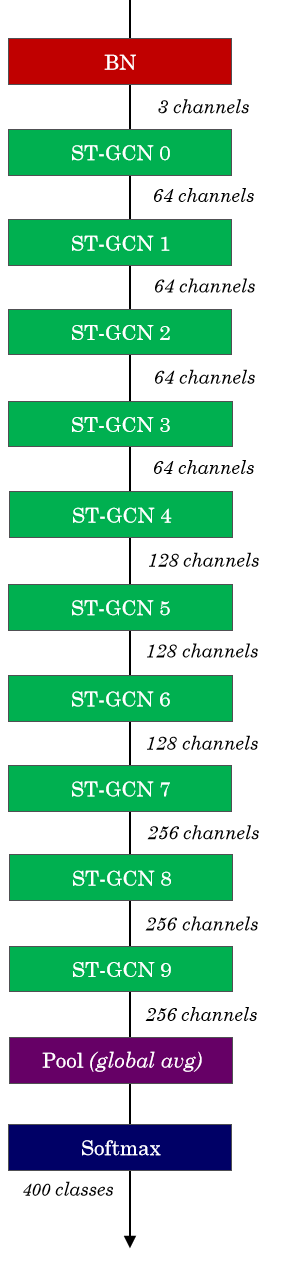
\includegraphics[width=2.5cm]{images/st_gcn_architecture}
    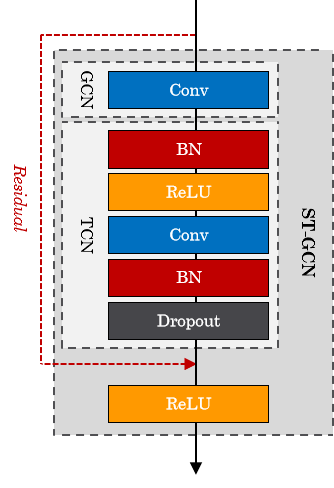
\includegraphics[width=3.0cm]{images/st_gcn_architeture_unit}
    \caption{Model architecture (left) and detail of a convolutional unit (right). ST-GCN units apply normalization, convolution, activation, and dropout operations to the graphs and take into account the residual value of the previous layer to calculate the output activations. Adapted from \cite{st-gcn-2018}.}
    \label{fig:st-gcn-architecture}
\end{figure}

To estimate the skeletons of individuals in videos, in \cite{st-gcn-2018} the authors used a library called OpenPose\footnote{
    Available at \url{https://github.com/CMU-Perceptual-Computing-Lab/openpose}.
}. It is an open-source tool that uses deep learning algorithms to detect and estimate up to 135 points from the human body \cite{cao-realtime-2017, simon-hand-2017, wei-cpm-2016}. Despite this, they only adopted 18 of these points, which correspond to the main body joints (see figure \ref{fig:keypoints-pose}).

% Para realizar a extração dos esqueletos a partir de vídeos contendo ações de indivíduos, em \cite{st-gcn-2018} os autores utilizaram uma biblioteca denominada OpenPose\footnote{
%    Disponível em \url{https://github.com/CMU-Perceptual-Computing-Lab/openpose}.
%}. Trata-se de uma ferramenta de código aberto que utiliza algoritmos de aprendizagem profunda para detectar e estimar até 135 pontos dos esqueletos de indivíduos em vídeos \cite{cao-realtime-2017, simon-hand-2017, wei-cpm-2016}. Apesar disso, os autores utilizaram apenas 18 desses pontos, os quais se correspondem às articulações principais do corpo (vide figura \ref{fig:keypoints-pose}). 

\image
	[3cm]
    {fig:keypoints-pose}
    {images/keypoints_pose_COCO_18}
    {Representation of the 18 points referring to the human body, extracted by OpenPose \cite{openpose-output-2018}.}

% Todo o fluxo descrito até aqui trata da aplicação do ST-GCN para o contexto onde vídeos isolados são gravados previamente e utilizados como entrada. Apesar disso, entende-se que seria possível, com algum trabalho adicional, evoluí-lo na direção de substituir essa entrada por um \textit{streaming} de vídeo capturado em tempo real por uma câmera. Para isso, seria necessário passar a estimar continuamente com uma biblioteca ou \textit{hardware} específico as poses dos \textit{frames} capturados, provendo assim um \textit{streaming} de esqueletos para o modelo. A biblioteca OpenPose (que está descrita em detalhes mais adiante) é capaz de atender a essa necessidade, porém seus requisitos de \textit{hardware} robusto podem acabar por limitar sua adoção em alguns contextos na prática. A leitura dos dados pelo modelo também precisaria ser evoluída afim de que ao invés de considerar informações em arquivos físicos, sejam utilizadas aquelas fornecidas pelo \textit{streaming} de esqueletos. Como o ST-GCN hoje só trabalha com vídeos de tamanho fixo, essa entrada em fluxo contínuo apenas seria classificada por ele de janelas em janelas de tempo, quando completado em memória esse número fixo estabelecido de \textit{frames}.


\section{Experiments} %%%%%%%%%%%%%%%%%%%%%%%%%%%%%%%%%%%%%%%%%%%%%%%%%%%%%%%%%%%%%%%%%%%%%%%
\label{sec:experimentos}

This section presents the approach used to organize and conduct the experiments in this work. 

First, the ST-GCN was chosen as the model for its ability to focus primarily on human body movement, disregarding external environment interference, as best addressed in sections \ref{sec:introducao} and \ref{sec:trabalhos-relacionados}. These aspects are essential for techniques that propose to address the recognition of sign language, which also has as one of its central elements the body dynamics. 

% Esta seção define a abordagem utilizada para organizar e conduzir os experimentos deste trabalho. Em primeiro lugar, foi estabelecido como modelo o ST-GCN devido à capacidade de centrar sua atenção essencialmente no movimento corpo humano, desconsiderando a interferência do ambiente externo, conforme abordam as seções \ref{sec:introducao} e \ref{sec:trabalhos-relacionados}. Entende-se que esses aspectos são essenciais para que uma técnica aborde o reconhecimento da língua de sinais, que também possui como elemento principal o corpo humano e sua dinâmica.

Next, the reference dataset to be used has been established, as well as the preprocessing steps required to create a new ST-GCN compliant set, according to the domain of the problem addressed here. Finally, small adjustments were made to the model and the training to collect the results of this method was conducted.

% Em seguida, foi estabelecido o \textit{dataset} a ser utilizado como referência, bem como as etapas de pré-processamento necessárias para criar uma novo conjunto compatível com o ST-GCN dentro dos objetivos deste trabalho. Por fim, foram realizados pequenos ajustes no modelo e conduzidos os treinamentos para coleta dos resultados deste trabalho.



\subsection{Dataset} %%%%%%%%%%%%%%%%%%%%%%%%%%%%%%%%%%%%%%%%%%%%%%%%%%%%%%%%%%%%%%%%%%%%%%%%%%%%%%%%%
\label{sec:dataset}

For this work was chosen the American Sign Language Lexicon Video Dataset (ASLLVD). It consists of a large public dataset\footnote{
   Available at \url{http://csr.bu.edu/asl/asllvd/annotate/index.html}.
} containing video sequences of thousands of American Sign Language (ASL) signs, as well as their annotations, respective start and end frame markings, and class labels for each sample \cite{ athitsos-asllvd-2008, neidle-2012, vloger-2012}.

% Foi selecionado para este trabalho o \textit{American Sign Language Lexicon Video Dataset} (ou ASLLVD). Ele consiste num \textit{dataset} público\footnote{
%   Disponível em \url{http://csr.bu.edu/asl/asllvd/annotate/index.html}.
%} amplo que contém sequências de vídeos de milhares de sinais distintos da Língua de Sinais Americana (\textit{American Sign Language}, ou ASL), bem como as anotações dessas sequências, os \textit{frames} de início e fim, e os rótulos de classe para cada sinal \cite{athitsos-asllvd-2008, neidle-2012, vloger-2012}.

According to the authors, each sign is articulated by native individuals in ASL, and video sequences are collected using a four-camera system that simultaneously captures two frontal views, one side view and one enlarged view of the face of these individuals. Figure \ref{fig:asllvd-example} exemplifies capturing three of these views for the "MERRY-GO-ROUND" sign. 

% Segundo os autores, cada sinal é articulado por indivíduos nativos da ASL, e as sequências de vídeo são coletadas utilizando um sistema de quatro câmeras que captura simultaneamente duas vistas frontais, uma vista lateral e uma vista ampliada da face desses indivíduos. A figura \ref{fig:asllvd-example} exemplifica a captura de três dessas vistas para o sinal "\textit{MERRY-GO-ROUND}".

\image
    {fig:asllvd-example}
    {images/asllvd_example}
    {Example of capture for the "MERRY-GO-ROUND" sign from three different perspectives, in the ASLLVD \cite[p. 2]{athitsos-asllvd-2008}.}
    
The number and type of signs included in ASLLVD are similar in scale and scope to the set of lexical entries in existing English-to-ASL dictionaries. There is at least one example of video per sign for almost all those contained in the Gallaudet Dictionary of American Sign Language \cite{athitsos-asllvd-2008, gallaudet-2005}.

% Ainda de acordo com os autores, o número e o tipo de sinais incluídos no ASLLVD são semelhantes em escala e escopo ao conjunto de entradas lexicais nos dicionários existentes de "Inglês-para-ASL". Existe ao menos um exemplo de vídeo por sinal para quase todos os sinais contidos no Dicionário Gallaudet de Língua Americana de Sinais \cite{athitsos-asllvd-2008, gallaudet-2005}, os quais são articulados por indivíduos nativos. 

By analyzing the dataset in detail it is possible to identify the existence of a total of 2,745 signs, represented in approximately 10 thousand samples. Each sign contains between 1 and 18 samples articulated by different individuals (where 4 is the average number of samples per sign).

% Ao analisar o \textit{dataset} em detalhe é possível identificar a existência de um total de 2.745 sinais, representados em aproximadamente 10 mil amostras. Cada sinal contém entre 1 e 18 amostras articuladas por diferentes indivíduos (sendo 4 o número médio de amostras por sinal).


\subsection{Creation of skeleton dataset for sign language} %%%%%%%%%%%%%%%%%%%%%%%%%%%%%%%%%%%%%%%%%%%%%%%%%%%%%%%%%%%%%%%%%%%%%%%%%%%
\label{sec:criacao-dataset}

In order to make the ASLLVD samples compatible with the input expected by the ST-GCN model it was necessary to apply a series of preprocessing steps, which gave rise to the new dataset containing the skeleton estimate for all individuals and signs contained therein.

% Para tornar as amostras do ASLLVD compatíveis com a entrada esperada pelo modelo ST-GCN foi necessário aplicar uma série de etapas de pré-processamento, as quais deram origem ao novo \textit{dataset} contendo a estimativa de esqueletos para todos os indivíduos e sinais contidos nele.

This new dataset was named \textbf{ASLLVD-Skeleton}, and has been made publicly available\footnote{
   Available at \url{http://www.cin.ufpe.br/~cca5/asllvd-skeleton}
} in order to contribute to the development of future studies on the recognition of sign languages.

% A esse novo \textit{dataset} foi atribuído o nome \textbf{ASLLVD-Skeleton}, e o mesmo foi disponibilizado publicamente\footnote{
%    Disponível em \url{http://www.cin.ufpe.br/~cca5/asllvd-skeleton}
%} com o intuito de contribuir com o desenvolvimento de estudos futuros no reconhecimento de línguas de sinais.

The steps applied to create this dataset are shown in figure \ref{fig:preprocessamento}, and described below.

% As etapas aplicadas na criação desse novo \textit{dataset} estão apresentadas na figura \ref{fig:preprocessamento} e descritas a seguir.

\image
    [8.5cm]
    {fig:preprocessamento}
    {en/images/dataset_preprocessing}
    {Preprocessing steps for creating the ASLLVD-Skeleton dataset.}

The first one consists in a preliminary step of \textbf{obtaining the videos} that make up the ASLLVD, in order to reconstitute it and make feasible the later stages. A metadata file contained in this dataset was used to guide this process. At this moment, only the videos captured by the frontal camera were considered, once they simultaneously contemplates movements of the trunk, hands and face of individuals.

% A primeira etapa consiste num passo preliminar de \textbf{obtenção dos vídeos} que compõem o ASLLVD de forma automática, afim de reconstitui-lo e viabilizar as etapas posteriores. Um arquivo de metadados\footnote{
%    Disponível em \url{http://www.bu.edu/asllrp/dai-asllvd-BU_glossing_with_variations_HS_information-extended-urls-RU.xls}
%} desse \textit{dataset} foi utilizado para guiar esse processo. Nesse momento foram considerados apenas os vídeos capturados pela câmera frontal, que contempla simultaneamente os movimentos do tronco, mãos e face dos indivíduos.

The next step is to \textbf{segment the videos} to generate a video sample for each signal. Every file in the original dataset corresponds to a section where multiple signs were recorded per individual. Due to this, it is necessary to constitute a new set organized in such a way that each sign is arranged individually with its respective label. For this, we also considered the metadata file discussed above, which has the labels and the start and end frame markings to perform the segmentation for each sign. The output of this step consists of small videos with average duration up to 5 seconds and looking similar to the one shown in figure \ref{fig:sign-original}.

% A etapa seguinte consiste em \textbf{segmentar os vídeos} para que seja obtido um vídeo por sinal. Isso se faz necessário porque cada arquivo no \textit{dataset} original corresponde a uma seção onde foram gravados múltiplos sinais por indivíduo. Com isso, é necessário constituir um novo conjunto organizado de tal forma que cada sinal esteja disposto individualmente com seu respectivo rótulo. Para isso, também foi considerado o arquivo de metadados comentado acima, que dispõe dos rótulos e das respectivas marcações de \textit{frames} de início e término para cada sinal nas seções. Como saída dessa etapa, tem-se pequenos vídeos com duração média de 1 a 5 segundos e com aspecto semelhante ao ilustrado na figura \ref{fig:sign-original}.

\image
    [4cm]
    {fig:sign-original}
    {images/sign_original}
    {Representation of the "EXAGGERATE" sign, segmented from the sections recorded in ASLLVD.}

The third step consists of \textbf{estimating the skeletons} of the individuals present in the segmented videos. In other words, at this moment the coordinates of the individuals' joints will be estimated for all frames, composing the skeletons that will give rise to the graphs used by the ST-GCN. In the same way as in \cite {st-gcn-2018}, we used the OpenPose library in this process. The difference, however, lies in the fact that in addition to the coordinates referring to the body, a considerably larger number of coordinates have been adopted here to also cover the hands and face of these individuals. In total there are 130 points, of which 21 correspond to each of the hands; 70 correspond to the face coordinates; and 18 correspond to the body (see figures \ref{fig:keypoints-face-hand} and \ref{fig:keypoints-pose}). Figure \ref{fig:sign-pose} illustrates the reconstruction in a 2D image of the coordinates estimated by OpenPose for the "EXAGGERATE" sign.

% O terceiro passo consiste em realizar a \textbf{estimar os esqueletos} dos indivíduos presentes em cada vídeo segmentado. Em outras palavras, nesse momento são extraídas as coordenadas das articulações desses indivíduos, \textit{frame} a \textit{frame}, para compor os esqueletos que darão origem aos grafos utilizados pelo ST-GCN. Para isso, da mesma forma como em \cite{st-gcn-2018}, utilizou-se a biblioteca OpenPose. A diferença, no entanto, está no fato de que além das coordenadas referentes ao corpo, aqui foi adotado um número consideravelmente maior de coordenadas para abranger também as mãos e face dos indivíduos. No total são 130 pontos, dos quais 21 correspondem a cada uma das mãos; 70 correspondem às coordenadas da face; e 18 correspondem ao corpo (vide figura \ref{fig:keypoints-face-hand} e figura \ref{fig:keypoints-pose}). A figura \ref{fig:sign-pose}, por sua vez, ilustra a reconstrução em uma imagem 2D das coordenadas estimadas pelo OpenPose para o sinal "EXAGGERATE".


\begin{figure}[ht]
    \centering
    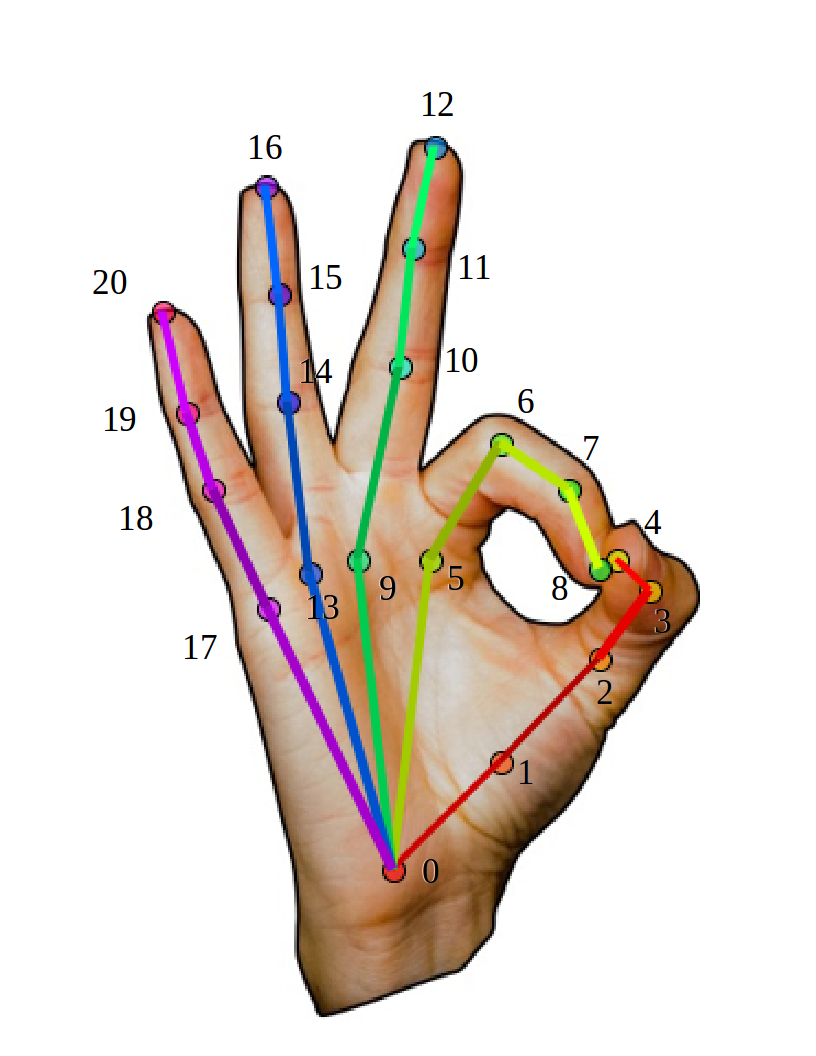
\includegraphics[width=2.5cm]{images/keypoints_hand}
    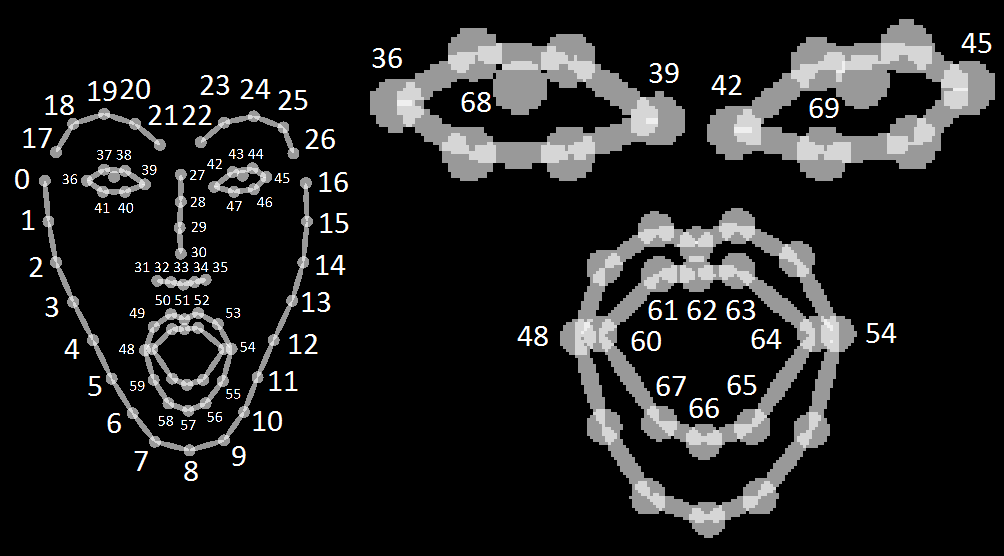
\includegraphics[width=4cm]{images/keypoints_face}
    \caption{Representation of the 21 points of the hand (left) and 70 points of the face (right) extracted by OpenPose \cite{openpose-output-2018}.}
    \label{fig:keypoints-face-hand}
\end{figure}

\begin{figure}[ht]
    \centering
    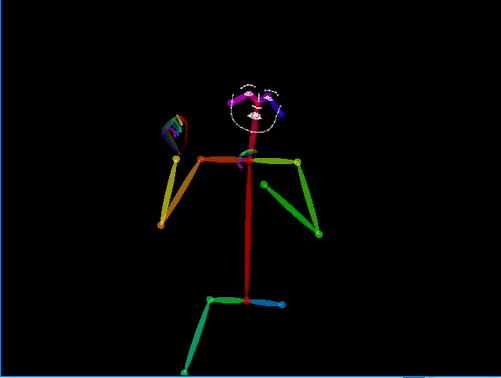
\includegraphics[width=3.5cm]{images/sign_pose}
    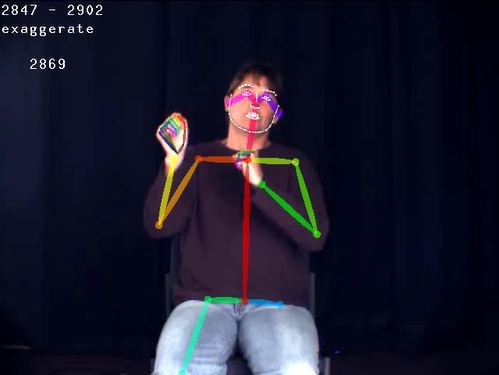
\includegraphics[width=3.5cm]{images/sign_pose_blended}
    \caption{Reconstruction of the skeleton from the coordinates estimated by OpenPose for the sign "EXAGGERATE" (left); and overlap of this skeleton in the original video (right).}
    \label{fig:sign-pose}
\end{figure}

Figure \ref{fig:openpose-coordinates} shows an example file obtained at the end of this step. In each frame, a section called "pose" with the coordinates of the X and Y axes estimated for  the body joints is contained, and a section "score" with the degree of confidence for each of these joints is also included.

% A figura \ref{fig:openpose-coordinates} mostra um exemplo de arquivo obtido ao final dessa etapa. Nele estão contidos para cada \textit{frame} uma seção denominada \textit{pose} com as coordenadas dos eixos X e Y estimadas para cada articulação do corpo, e uma seção \textit{score} que contempla o grau de confiança para a estimativa de cada uma dessas articulações..

\image
    [7.5cm]
    {fig:openpose-coordinates}
    {images/openpose_coordinates}
    {Example file containing the estimated coordinates for the skeletons in a sign. It includes a "pose" section with the X and Y coordinates of the estimated joints, and a "score" section with the respective degrees of confidence for each of them.}

The fourth step concerns the \textbf{division of the dataset} processed so far into smaller subsets that will be used for training and testing the model. For this procedure, a cross-validation dataset tool called "\textit{train\_test\_split}", which is made available by the Scikit-Learn \cite{scikit-learn} library, was used. In this division, a proportion of 80\% of the samples were assigned for training (corresponding to 7,798 items) and 20\% for tests (corresponding to 1,950 items). This is a commonly adopted proportion and we understand that the number of samples in these groups is sufficient to validate the performance of most machine learning models.

% A quarta etapa diz respeito à \textbf{divisão do \textit{dataset}} processado até aqui em subconjuntos menores que serão utilizados para o treinamento e testes do modelo. Para esse procedimento, foi utilizada uma ferramenta de divisão de \textit{datasets} para validação cruzada denominada "\textit{train\_test\_split}", que é disponibilizada pela biblioteca Scikit-Learn \cite{scikit-learn}. Nessa divisão, foi considerada uma proporção de 80\% das amostras para treinamento (que corresponde a 7.798 itens) e 20\% para testes (correspondendo a 1.950 itens). Essa é uma proporção comumente adotada e entende-se que o número de amostras separadas para cada etapa é suficiente para validar o desempenho da grande parte dos modelos de aprendizagem de máquina.

Finally, the fifth step is to \textbf{normalize and serialize} the samples in order to make them compatible with the ST-GCN reading format. Normalization aims to make the length of all samples uniform by applying repetition of their frames sequentially to the complete filling of an established fixed number of frames. The number of fixed frames adopted here is 63 (which at a rate of 30 FPS, corresponds to a video with an approximate duration of 2 seconds). Serialization, in turn, consists of preloading the normalized samples from the subsets created above to translate them into physical Python \cite{python} files, which contain their in-memory representations. This is the format used by the ST-GCN, and it is adopted to optimize the process of data loading. For each of the subsets divided in the previous step two physical files are generated: one containing the samples and other containing the labels for those samples.

%Por fim, a quinta etapa consiste em \textbf{normalizar e serializar} as amostras afim de torná-las compatíveis com o formato de leitura do ST-GCN. A normalização objetiva tornar o comprimento de todas as amostras uniforme, aplicando para isso a repetição de seus \textit{frames} de forma sequencial até o preenchimento completo de um número fixo estabelecido de \textit{frames}. O número aqui adotado é de 63 \textit{frames} (que a uma taxa de 30 FPS, corresponde a um vídeo de duração aproximada de 2 segundos). A serialização, por sua vez, consiste em pré-carregar as amostras dos subconjuntos criados acima para traduzi-las em arquivos físicos do Python \cite{python}, contendo as respectivas representações em memória desses objetos. Esse é o formato de entrada esperado pelo ST-GCN, que é adotado para otimizar o processo de leitura dos dados. Para cada subconjunto acima são criados dois arquivos físicos: um contendo sua lista de amostras e outro contendo a lista de rótulos para essas amostras. 

The output of the processing of each of the above steps is made available individually in ASLLVD-Skeleton, as above. The source code that performs the processing of these steps is also available along with the ST-GCN adaptations detailed in the following section.

% O resultado do processamento de cada uma das etapas acima está disponibilizado individualmente no ASLLVD-Skeleton, conforme acima. O código fonte que realiza o processamento dessas etapas, por sua vez, está disponível juntamente com as adaptações do ST-GCN, conforme seção a seguir.


\subsection{ST-GCN adaptation for the recognition of sign language} %%%%%%%%%%%%%%%%%%%%%%%%%%%%%%%%%%%%%%%%%%%%%%%%%%%%%%%%%%%%%%%%%%%%%%%%%%%
\label{sec:adaptacao-st-gcn}

Since the graph representation approach adopted by the ST-GCN is very flexible, it was not necessary in this work to make modifications in the architecture of the model. Instead, only punctual adaptations to get him to consider the new coordinates for the sign language domain were required.

% Uma vez que a abordagem de representação por meio de grafos adotada pelo ST-GCN é bastante flexível, não foi necessário neste trabalho realizar modificações na arquitetura do modelo. Ao invés disso, apenas adaptações pontuais para fazer com que ele passasse a considerar as novas coordenadas para o domínio da língua de sinais foram realizadas. 

Thus, a new graph layout for this problem was created, contemplating the 130 joints adopted here and their relations. In addition, adjustments were made on the matrices used in the training and test data reader in order to accommodate the dimensions of the new coordinates.

% Dessa forma, foi criado um novo \textit{layout} de grafo para o problema atual, denominado "openpose-sl" contemplando as 130 articulações e suas relações. Além disso, foi necessário realizar ajustes nas dimensões de matrizes utilizadas no mecanismo de leitura dos dados para possibilitar com que eles comportassem as novas dimensões.

The source code containing these adaptations has been made publicly available\footnote{
    Available at \url{http://www.cin.ufpe.br/~cca5/st-gcn-sl}
}. This code consists of a \textit{forked} repository created from the one originally developed by the authors in \cite{st-gcn-2018}.

%O código fonte contendo essas adaptações, bem como a implementação da sequência completa de etapas de pré-processamento está disponível publicamente\footnote{
%    Disponível em \url{http://www.cin.ufpe.br/~cca5/st-gcn-sl}
%}. Esse código consiste num \textit{fork} criado a partir daquele originalmente desenvolvido pelos autores em \cite{st-gcn-2018}.



\subsection{Preparation of experiments} %%%%%%%%%%%%%%%%%%%%%%%%%%%%%%%%%%%%%%%%%%%%%%%%%%%%%%%%%%%%%%%%%%%%%%%%%%%
\label{experimentos}

In this work, we adopted as reference the experiments presented in \cite{lim-2016}, which evaluate the performance in recognition of the ASLLVD dataset by the Block-Based Histogram of Optical Flow (BHOF) method (see section \ref{sec:trabalhos-relacionados}) and also by popular techniques such as Motion Energy Image (MEI) \cite{athitsos-asllvd-2008}, Motion History Image (MHI) \cite{babu-2004}, Principal Component Analysis (PCA) \cite{dreuw-2012} and Histogram of Optical Flow (HOF) \cite{laptev-2008}.

% Para este trabalho, foram utilizados como referência os experimentos apresentados em \cite{lim-2016}, o qual avalia a performance do reconhecimento dos sinais no \textit{dataset} ASLLVD pela técnica BHOF (vide seção \ref{sec:trabalhos-relacionados}) e também por técnicas populares como \textit{Motion Energy Image} (MEI) \cite{athitsos-asllvd-2008}, \textit{Motion History Image} (MHI) \cite{babu-2004}, \textit{Principal Component Analysis} (PCA) \cite{dreuw-2012} e \textit{Histogram of Optical Flow} (HOF) \cite{laptev-2008}. 

For this purpose, the authors used a subset containing 20 signs selected from the ASLLVD, as presented in table \ref{tab:asllvd-20}. To reproduce this configuration, the skeletons estimated for these signs were selected from the ASLLVD-Skeleton dataset created in section \ref{sec:criacao-dataset}. Once the resulting number of samples is small, totaling 185 items, it was necessary to apply a new division making 77\% of this subset to be separated for training and 33\% for tests. With this, a greater balance in the number of samples was obtained for an adequate evaluation of the model. Finally, as a new division of the samples was made, it was also necessary to normalize and serialize them to be compatible with the ST-GCN. In this process the same procedure as in section \ref{sec:criacao-dataset} was performed. The resulting subset was made publicly available\footnote{
    Available at \url{http://www.cin.ufpe.br/~cca5/asllvd-skeleton-20}
} and is called \textbf{ASLLVD-Skeleton-20}.

% Com esse propósito, os autores utilizaram um subconjunto contendo 20 sinais selecionados a partir do ASLLVD, conforme apresenta a tabela \ref{tab:asllvd-20}. Para reproduzir essa configuração, foram selecionadas as poses com esqueletos estimados para esse sinais a partir do \textit{dataset} criado na seção \ref{sec:criacao-dataset}. Como o número resultante de amostras é pequeno, totalizando 185 itens, foi necessário aplicar uma nova divisão fazendo com que 77\% desse subconjunto fosse separado para treinamento e 33\% para testes. Com isso, obteve-se um equilibrar maior no número de amostras uma avaliação mais adequada do modelo. Por fim, uma vez que tem-se uma nova divisão, foi necessário normalizar e serializar os novos suconjuntos para compatibilizá-los com o ST-GCN. Nesse processo adotou-se o mesmo procedimento apresentado na seção \ref{sec:criacao-dataset}. O subconjunto resultante, denominado de \textbf{ASLLVD-Skeleton-20} também foi disponibilizado publicamente\footnote{
%    Disponível em \url{http://www.cin.ufpe.br/~cca5/asllvd-skeleton-20}
%}.

\begin{table}[ht]
\caption{Selected signs for the experiments in \cite{lim-2016}.}
\label{tab:asllvd-20}
\begin{tabular}{ll}
\hline
Dataset & Selected signs \\ \hline
ASLLVD & \begin{tabular}[c]{@{}l@{}}adopt, again, all, awkward, baseball, behavior, can, chat, \\ cheap, cheat, church, coat, conflict, court, deposit, depressed, \\ doctor, don’t want, dress, enough\end{tabular} \\ \hline
\end{tabular}
\end{table}

Still due to the characteristics of this small dataset, the size of the batch used in the training had to be reduced so that better results could be observed in the experiments. Thus, after a few failed attempts with larger batches, a batch size of 8 samples was considered.

%Ainda devido às características desse conjunto de dados pequeno, o tamanho do \textit{batch} utilizado para o treinamento precisou ser reduzido para que melhores resultados passassem a ser observados nos experimentos. Dessa forma, após algumas tentativas frustradas com \textit{batches} maiores, passou-se a considerar um tamanho de 8 amostras.

In the same way as in the original implementation of the ST-GCN training algorithm in \cite {st-gcn-2018}, the experiments in this work used as optimizer the Stochastic Gradient Descent (SGD) with Nesterov Momentum, which in turn is able to improve stability and the convergence of the SGD, as described by \cite{stanford-2018, bengio-2013, sutskever-2013}.

% Da mesma forma como na implementação original do algoritmo de treinamento do ST-GCN em \cite{st-gcn-2018}, os experimentos deste trabalho utilizaram como método de otimização o Gradiente Descendente Estocástico (ou \textit{Stochastic Gradient Descent} - SGD) com Momento de Nesterov, que por sua vez é capaz de melhorar a estabilidade e a convergência do SGD, como descrevem \cite{stanford-2018, bengio-2013, sutskever-2013}.

For the learning rate, a strategy of initializing it with a high value was applied in order that the random weights are placed in the direction of convergence within the first epochs. Then, this rate was gradually reduced in later epochs, allowing for more and more refined adjustments of training weights. Thus, in the experiment with the 20 selected signs, a total of 600 epochs were used, adopting an initial rate of 0.1, which was decreased to values of 0.01, 0.001, 0.0001 and 0.00001 after the end of the epochs 50, 250, 350 and 450, respectively.

% Para a taxa de aprendizagem, foi aplicada uma estratégia de inicializa-la com um valor elevado afim de que os pesos aleatórios sejam colocados na direção de convergência dentro das primeiras épocas. Em seguida, essa taxa foi reduzida gradativamente nas épocas posteriores possibilitando ajustes cada vez mais refinados dos pesos no treinamento. Dessa forma, no experimento com os 20 sinais selecionados foi utilizado um total de 600 épocas adotando uma taxa inicial de 0.1, a qual foi decaída para os valores de 0.01, 0.001, 0.0001 e 0.00001 após o término do treinamento das épocas 50, 250, 350 e 450, respectivamente.

% TODO: revisar configurações do experimento

In addition to training with the subset of 20 signs above, an experiment with the complete ASLLVD dataset was also conducted in order to establish a reference value for it. To do this, only the settings related to the batch size and the decay epochs of the learning rate had to be changed. Thus, the new batch size for this scenario with 2.745 signs was 24 and the learning rate had similar behavior to the experiment above, being decayed at the end of the epochs 100, 300, 400 and 500.

% Além do treinamento com o subconjunto de 20 sinais, também foi conduzido um experimento com o \textit{dataset} completo do ASLLVD, afim de estabelecer um valor de referência para ele. Para isso, apenas as configurações relacionadas ao tamanho do \textit{batch} e das épocas de decaimento da taxa de aprendizado precisaram ser alteradas. Sendo assim, o novo tamanho de \textit{batch} para esse cenário com muito mais amostras foi de 24 e a taxa de aprendizado teve comportamento de decaimento igual ao contexto acima, sendo aplicado ao término das épocas 100, 300, 400 e 500.

The results obtained in both scenarios are presented in the following section, and the pre-trained models are available together with the adaptations in the ST-GCN, according to section \ref{sec:adaptacao-st-gcn}.

% Os resultados obtidos em ambos os cenários estão apresentados na seção a seguir, e os modelos pré-treinados resultantes estão disponibilizados juntamente com as adaptações no ST-GCN, conforme seção seção \ref{sec:adaptacao-st-gcn}.


\section{Results} %%%%%%%%%%%%%%%%%%%%%%%%%%%%%%%%%%%%%%%%%%%
\label{sec:resultados}

This section presents the findings and results obtained from the application of the approach described in the this work.

% Esta seção apresenta as descobertas e resultados obtidos a partir da aplicação da abordagem descrita nas seções anteriores. 

The first experiment was performed using the approach presented in \cite{lim-2016}, which considers the selection of 20 specific signs of the ASLLVD, whose performance is represented in figure \ref{fig:training-asllvd-20}. The red line presents the accuracy of the model (\textit{top-1}), and its evolution over the course of training epochs. The gray line represents the \textit{top-5} accuracy, which corresponds to the accuracy based on the 5 most likely responses presented by the model. Finally, the blue dashed line represents the evolution of the learning rate used in the respective epochs, and its decay behavior.

% O primeiro experimento foi realizado utilizando a abordagem apresentada em \cite{lim-2016}, que considera a seleção de 20 sinais específicos do ASLLVD, e cujo desempenho está representado na figura \ref{fig:training-asllvd-20}. A linha vermelha apresenta a acurácia (\textit{top-1}) do modelo, e exibe sua evolução no decorrer das épocas de treinamento. Na linha cinza está representada a acurácia \textit{top-5}, que corresponde à acurácia com base nas 5 respostas de maior probabilidade apresentadas pelo modelo. Por fim, a linha tracejada azul representa evolução da taxa de aprendizagem utilizada nas respectivas épocas, e seu comportamento de decaimento.

\image
    [8.5cm]
    {fig:training-asllvd-20}
    {images/results_20}
    {Accuracy obtained by the presented approach in the recognition of the 20 signs selected from the ASLLVD. The red line represents the \textit{top-1} accuracy during the training periods; the gray line, the \textit{top-5} accuracy; and the blue dashed line illustrates the learning rate and its decay in the respective epochs.}

It can be seen from the image that the model was able to consistently achieve an accuracy of 35.85\% from epoch 400 on sign recognition. The \textit{top-5} accuracy, in turn, was able to reach a number of 64.15\%. This performance was superior to that presented by traditional techniques such as MEI and MHI, but was not able to overcome the results obtained by techniques such as PCA and BHOF \cite{lim-2016}. Table \ref{tab:results-comparison-20} presents the comparison of these results with the proposed approach.

% Pode-se perceber pela imagem que o modelo conseguiu alcançar de forma consistente uma acurácia de 35,85\% a partir da época 400 no reconhecimento dos sinais. A acurácia \textit{top-5}, por sua vez, foi capaz de alcançar um número de 64,15\%. Esse desempenho foi superior ao apresentado por técnicas tradicionais como o MEI e o MHI, mas não foi capaz de superar os resultados obtidos por técnicas como o PCA e o BHOF \cite{lim-2016}. A tabela \ref{tab:results-comparison-20} apresenta a comparação desses resultados com a abordagem proposta.

\begin{table}[ht]
\centering
\caption{Accuracy in sign recognition using different approaches, as proposed in \cite{lim-2016}.}
\label{tab:results-comparison-20}
\begin{tabular}{lc}
\hline
                   & Accuracy (\%)  \\ \hline
MHI                & 10.00                     \\
MEI                & 25.00                     \\
\textbf{ST-GCN SL} & \textbf{35.85}            \\
PCA                & 45.00                     \\
HOF                & 70.00                     \\
BHOF               & 85.00                     \\ \hline
\end{tabular}
\end{table}


% TODO: revisar resultados do ASLLVD

In order to establish a reference with the complete ASLLVD dataset, a second experiment was performed using its 2,745 signs. In this scenario, an accuracy (\textit{top-1}) of 7.03\% and a \textit{top-5} accuracy of approximately 14.67\% was observed. Of course, this is a much more challenging task than the one proposed in \cite{lim-2016} and these results clearly reflect this complexity.

% Afim de estabelecer uma referência com o \textit{dataset} completo do ASLLVD, foi realizado um segundo experimento utilizado os seus 2.745 sinais. Nesse cenário, foi observada uma acurácia (\textit{top-1}) de 7,03\% e uma acurácia \textit{top-5} de aproximadamente 14,67\%. Certamente, trata-se de uma tarefa muito mais desafiadora do que a proposta em \cite{lim-2016} e os resultados obtidos refletem claramente essa complexidade. 

%\image
%    [8.5cm]
%    {fig:training-asllvd}
%    {images/results}
%    {Acurácia obtida no treinamento do \textit{dataset} completo ASLLVD. Na imagem estão ilustradas a acurácia Top 1, a acurácia Top 5 e a taxa de aprendizagem utilizada e seu decaimento no decorrer das épocas.}

Recapitulating the approach proposed in this paper, it is observable that one of its main strategies was to adopt a greater number of joints in order that parts of the body not originally considered in \cite{st-gcn-2018} (such as hands and face), would be adopted for the recognition of sign language, capturing different aspects of its dynamics. This caused the number of joints to increase by more than 7 times, from 18 to 130.

% Ao recapitular a abordagem proposta neste trabalho, percebe-se que uma de suas principais estratégias consiste em adotar um número maior de articulações afim de que partes do corpo não consideradas originalmente em \cite{st-gcn-2018}, como mãos e face, passassem a ser utilizadas para o reconhecimento da língua de sinais capturando diferentes aspectos de sua dinâmica. Isso fez com que o número de articulações aumentasse em mais de 7 vezes, partindo de 18 para 130. 

However, the results obtained in these experiments lead us to believe that many of these 130 points did not add significant information about the domain of the sign language problem to the model used. For example, when looking at some samples of ASLLVD presented in the previous sections, we will notice that individuals are always seated and this makes the coordinates related to their lower limbs not important; the face, in turn, comprises more than half of the coordinates used, but many of these points do not denote expressive movements for the signs or are redundant due to the high density of coordinates in that region.

% Contudo, os resultados obtidos nesses experimentos nos levam a acreditar que muitos desses 130 pontos não adicionaram informação significativa acerca do domínio do problema da língua de sinais para o modelo utilizado. Por exemplo, ao observar algumas amostras do ASLLVD apresentadas nas seções anteriores, perceberemos que os indivíduos estão sempre sentados e isso faz com que as coordenadas relacionadas a seus membros inferiores não sejam importantes; a face, por sua vez, contempla mais da metade das coordenadas utilizadas, porém muitos desses pontos não denotam movimentos expressivos para os sinais ou então são redundantes devido à grande densidade de coordenadas nessa região. 

In contrast, the BHOF \cite{lim-2016} aims to centralize the focus on hand movement by isolating them from the rest of the body and constructing histograms from the blocks in the frames where they are contained during articulation of the signs. Effectively, the hands describe some of the main features in sign language movements, and certainly the focus on them and the success in discarding little relevant information made this technique to present quite expressive results in relation to the current work. This technique is derived from the HOF and differs from it only by the approach of isolating the hands of individuals when calculating the optical flow histogram.

% Em contrapartida, o BHOF \cite{lim-2016} adota como objetivo centralizar o foco no movimento das mãos, isolando-as do restante do corpo e construindo histogramas a partir dos blocos nos \textit{frames} onde elas estão contidas durante a articulação dos sinais. De maneira efetiva, as mãos descrevem alguns dos principais traços nos movimentos da língua de sinais e, certamente o foco nelas e o sucesso em descartar informações pouco relevantes fizeram com que essa técnica apresentasse os resultados bastante expressivos com relação ao trabalho atual. Essa técnica é derivada do HOF e difere-se dele apenas pela abordagem de isolar as mãos dos indivíduos ao calcular o histograma do fluxo óptico.


Methods such as MEI and MHI present more primitive approaches, which basically detect the movements and their intensity from the difference between the consecutive frames of actions. They are not able to differentiate individuals or to focus on specific parts of their body, causing movements of any nature to be considered equivalently. The PCA, in turn, adds the ability to reduce the dimensionality of the components based on the identification of those with greater variance and that, consequently, are more relevant for the detection of movement in the frames.

% Métodos como o MEI e MHI apresentam abordagens mais primitivas, que basicamente detectam os movimentos e sua intensidade a partir da diferença entre os \textit{frames} consecutivos das ações. Eles não são capazes de diferenciar indivíduos ou de focar em partes específicas de seu corpo, fazendo com que movimentos de qualquer natureza sejam considerados de maneira equivalente. O PCA, por sua vez, adiciona a capacidade de reduzir a dimensionalidade dos componentes utilizados com base na identificação daqueles de maior variância e que, consequentemente, são mais relevantes para a identificação do movimento nos \textit{frames}. 

Although the results obtained with the presented approach did not reach an expressive performance like the BHOF, it is able to point the direction for the development of new studies. For future work, it is understood that there is a need for a revision in the number of coordinates used, possibly leading to an assessment in the potential of each group to add significance to the domain of sign language recognition.

% Apesar dos resultados obtidos com a abordagem apresentados não terem alcançado um desempenho expressivo como o BHOF, que ele é capaz de apontar a direção para o desenvolvimento de novos estudos. Para trabalhos futuros, entende-se que há a necessidade de uma revisão no número de coordenadas utilizadas, eventualmente conduzindo uma avaliação do potencial de cada grupo delas em adicionar significância acerca do domínio do reconhecimento da língua de sinais.


% Bibliografia
\bibliographystyle{IEEEtran}
\bibliography{IEEEabrv,references.bib}

\end{document}
